\nonstopmode
\documentclass[12pt,a4paper,english]{article}
\usepackage{amsmath}
\usepackage{url}
\usepackage{graphicx}
\usepackage[T1]{fontenc}
\usepackage[utf8]{inputenc}
\usepackage[british]{babel}
\usepackage{natbib}
\usepackage{csquotes}
\usepackage[titletoc]{appendix}
\usepackage{float}
\usepackage{amssymb}
\usepackage{datetime}
\usepackage{pdfpages}



\begin{document}
\ddmmyyyydate
\renewcommand{\dateseparator}{.}
\parskip 2mm
\parindent 0mm

\begin{titlepage}
  \setlength{\parindent}{0mm}
  \sloppy
  \large \textsc{University of Helsinki \\
				 Faculty of Social Sciences \\
                 Department of Political and Economic Studies \\
                 Economics}
  \vspace{5mm}

  \hrule height3pt
  \vspace{20mm}

  \begin{center}
    \large Master's thesis
    \linebreak \vfill   

    \huge \textbf{Unemployment Persistence \\ in the Eurozone} \\
    \vspace{2mm}
        \Large \textbf{Effects of Gender Differences in \\ Labour Market Behaviour}
    \vspace{20mm}

    \Large Matias Luukkanen \linebreak
    
    \vfill

  \end{center}
  \hrule height2pt
  \vspace{15mm}

  Supervisor: Markus Jäntti
  \hfill
  \today    
\end{titlepage}


\includepdf[pages={1}]{abstract.pdf}


\includepdf[pages={1}]{tiivistelma.pdf}
\setcounter{page}{1}
\tableofcontents
\clearpage
\renewcommand{\baselinestretch}{1.50}\normalsize
\section{Introduction}                                    

The global economic downturn, initiated by the financial crisis of 2007-2008, ended an era of stable growth with only moderate business cycle variation. Aggregate outputs plunged in virtually every developed country and high levels of unemployment lasted over several years. The long term effects of major shocks are likely to induce permanent decrease in potential output, not to mention the social and material costs of a lost generation of working aged people condemned to long-term unemployment and social exclusion. The purpose of this thesis is to study the persistence of the unemployment shock, and specifically to determine if the gender differences in labour market behaviour played a part.

The debate around the long-term effects of major shocks has focused on the Natural Rate of Unemployment (later NRU) and hysteresis narratives. The NRU was first formally proposed by \cite{phelps1967} and \cite{friedman1968}, who argue that aggregate output and unemployment have a natural equilibrium level towards which the economy self-adjusts after temporary shocks. Therefore, according to the theory of NRU, the optimal strategy for the policy maker is to provide an institutional framework that interferes with this self-adjustment as little as possible. 

The hysteresis narrative, on the other hand, considers the main property of shocks to be their persistence \citep{blanchard1987}. In its most strict interpretation, the level of unemployment is explained by the cumulative history of previous shocks: any shock to the economy leaves a permanent trace to all future realisations. The NRU is irrelevant if the persistence of this history is the main cause for the present level of unemployment and the deviation from the potential level of production. As a consequence, an appropriate policy response to a labour market with high persistence of unemployment is active monetary or fiscal stimulus to guide demand of labour to its optimal level. The hysteresis narrative is thus only concerned with the dynamics of \textit{how} a certain level of unemployment is reached, although the existence of an equilibrium level of unemployment is not ruled out. 

Whether unemployment has a stable natural rate or its dynamics are better accounted for by unit root structure has been studied in economic literature with varying outcomes. A general tendency has been to reject hysteresis in the US but not in Europe. This points to the institutional differences that affect unemployment dynamics, such as the unemployment insurance (UI) regime and the trade unions. It seems plausible that the suitability of either approach depends on the magnitude of the shock and various background factors that are determined by economic and social institutions. It is therefore reasonable to ask whether the European economic crisis is characterised by persistent unemployment and whether it can be formally modelled as a unit root time series, in which unity is a solution to the characteristic equation.

If persistence is strong enough, there may not be any practical difference between a stationary and an integrated process. The environmental factors that affect unemployment dynamics, such as the political and social climate, do change over time. That is why we are always dealing with the short term when investigating the dynamic properties of the subject at hand.

Investigation of a longer time-span cannot be justified, which results in a small number of observations. Furthermore, the low power of stationarity tests for shorter series, studying individual countries is relatively ineffective. That is why I am using a panel unit root test for all 11 original Eurozone countries\footnote{List of countries and corresponding abreviations used in the graphs later on are listed in Appendix \ref{countries}} decomposed by gender. 

Several researchers have done this and this

Cultural and historical reasons have forced men and women into different roles and labour market outcomes. Women are typically less attached to the labour force and the overall participation level among women is lower than among men \citep{gonzalo2000}. The are also distinct differences in types of professions and career paths \citep{arulampalam2007,blau2003}. The question that I intend to answer is whether these differences are big enough to cause an observable difference in the persistence of unemployment shocks.

The necessary data was retrieved from the OECD public database collected within the Labour Force Survey(LFS) under Eurostat coordination. For reasons concerning comparability of data across the countries in the analysis, I have decided to use only the 11 original Eurozone countries. The decision to exclude, for example, other European countries is based on the comparability of the institutional environment the countries are subject to. The fact that these countries are subject to the same monetary policy regime and parallel fiscal policy allow me to assume that all of the countries included are similar enough to be studied in a panel setting.

I use seasonally adjusted quarterly unemployment rates in the analysis. After an initial investigation of descriptives, I estimate an autoregressive (AR) time series model for each country and gender. Then I calculate the Augmented Dickey-Fuller(ADF) statistic for testing the null of a unit root. 

The individual statistics are combined using two different panel unit root tests. The first test I use is formulated by \cite{im2003} (later referred to as the IPS-test)and the other by \cite{maddala1999} (later, the MW-test). The panel statistics are calculated for each gender separately as well as for the aggregate data in order to determine possible differences.

Finally, I will present the estimation results and discuss them in the context of hysteresis versus NRU complemented with interpretation of the impulse response functions (IRF's) of the estimated AR models. The IRF's are calculated for the countries that present a weakly stationary unemployment history.

I will show that unemployment in the Eurozone is mainly characterized by an integrated model, with a few exceptions. Also, the rejection of the unit root is apparently driven by female unemployment. It is possible to conclude that the gender differences in labour market behaviour are significant to the question of hysteresis. This may be the outcome of differences in the distribution of workers between private and public sector as well as different hazard rates into non-participation.

Conclusions and policy implications are discussed in the final chapter.  Rather than trying to prove either the NRU or hysteresis as inapplicable, my intention is to maintain a conciliatory tone throughout the paper. Both of these narratives have their merits and provide unique insight into understanding how labour markets function and how we should regulate them. 

As the economic crisis drags on and governments are scrambling for effective remedies, the question about the relevance of counter cyclical financial policy is as great as ever. If indeed unemployment is characterised by high level of persistence over time, overlooking potentially effective means for actively steering production back to its potential path might prove to have dire consequences.


\clearpage
\section{NRU vs Hysteresis}
In this chapter I first review the historical discussion on the role of monetary policy, starting from the emergence of the NRU. This new addition to the theoretical toolbox for economic policy proved to be highly influential and resulted in a major shift in how the role of government in steering the economy was perceived. The hysteresis hypothesis marked the end of the period of undisputed success of the NRU interpretation for unemployment dynamics and provided new insight to the theory of equilibrium unemployment.

Furthermore, I present the basics of these theories and extract the relevant deductions that allow me to form the econometric model used in the analysis. Also the strength of the resulting conclusions is briefly discussed in the context of the theoretical background. I will also review the implications to determining correct policy responses to the business cycle.

Finally, In the last section of this chapter, I present the Non-Accelerating Inflation Rate Unemployment(NAIRU). It gives an empirical interpretation of the NRU and also highlights the complementary nature of the theoretical and historical quarrel.

\vspace{2cm}

\subsection{The Natural Rate of Unemployment}

At the time that \cite{friedman1968} and \cite{phelps1967} published their papers introducing the NRU, the dominant paradigm as basis for macroeconomic policy was the Phillips curve \citep{nelson2007}. A seemingly stable negative relationship between unemployment and inflation allowed economic policy to manipulate the unemployment level \citep{phillips1958}. For instance, if a policy maker wants to move unemployment from $U_1$ to $U_2$ as depicted in Figure~\ref{fig:phillipscurve1}, she needed to adjust inflation from $I_1$ to $I_2$.


\begin{figure}[h]
\vspace{1.5cm}
	\centering
	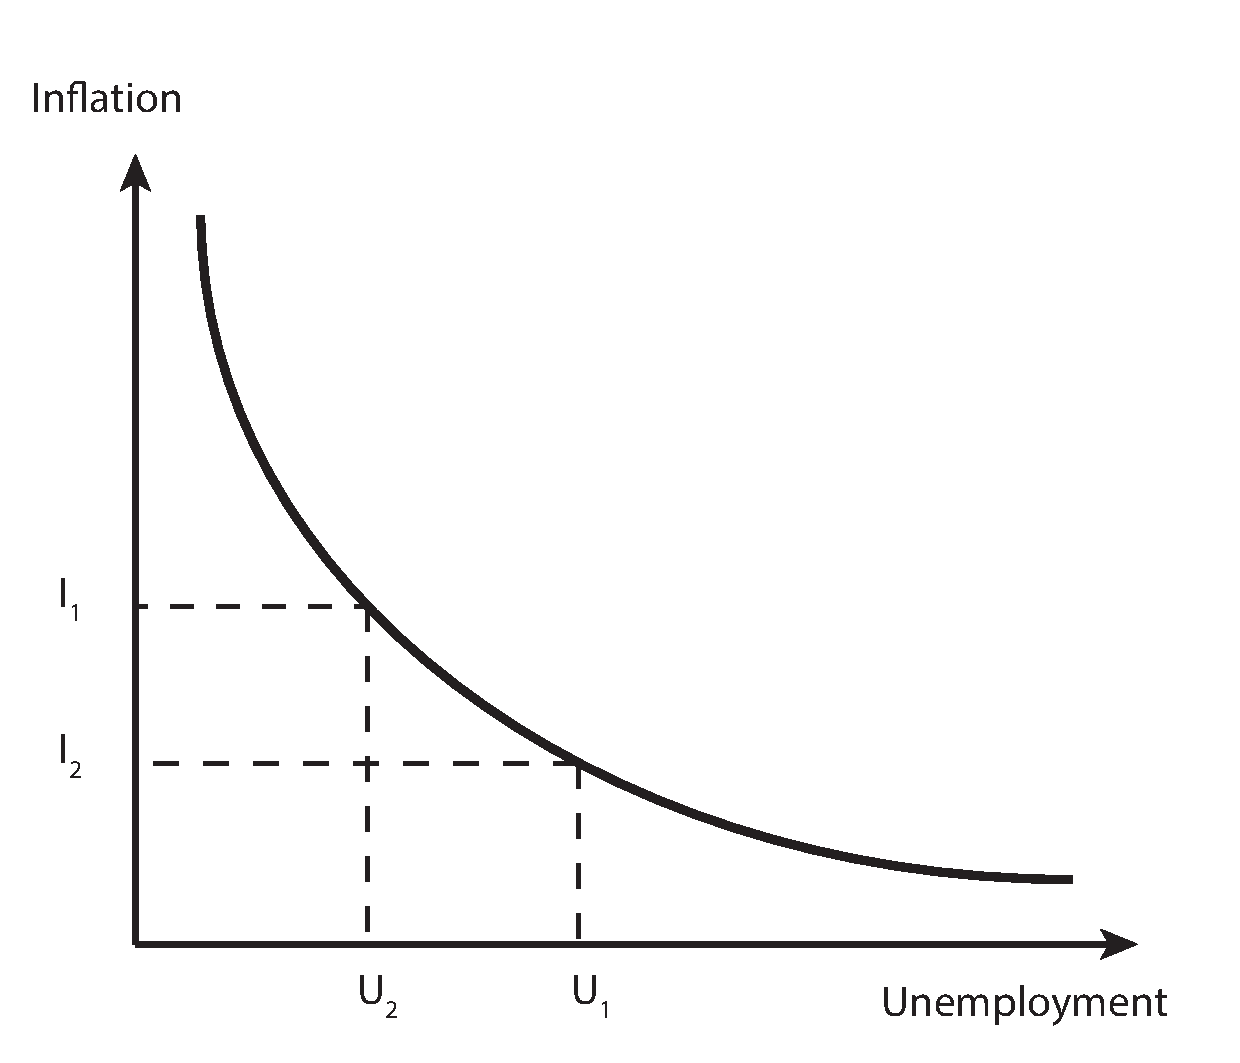
\includegraphics[width=0.75\linewidth]{Graphs/Phillips_curve_1}
	\caption{The Simple	 Phillips Curve}
	\label{fig:phillipscurve1}
\vspace{1.5cm}
\end{figure}


Empirical evidence for a stable Phillips curve did not materialize in the post-World War II world where governments were concentrating on maintaining full employment. An alternative idea started to emerge from the reasoning that if a stable inflation would be achieved, then everyone could adjust their current behaviour accordingly. If an employer could anticipate a certain change in prices, she could incorporate that insight into the wages, and the real effect in the demand would never materialize. This view was reinforced by the problems governments across the world were having with inflation, which threatened to spiral out of control.  \citep{friedman1977, nelson2007, blanchard1986}


\cite{friedman1968} and \cite{phelps1967} introduced their theory to complement the original Phillips curve by stating that the constant relationship only applies in the short run. Instead in the long run, the relationship between inflation and level of production alongside unemployment are independent of each other. This is because, the nominal shock to demand disappears when expectations about future inflation is adjusted to accommodate the effects of the shock. The Phillips curve would then shift accordingly.


\begin{figure}[h!]
\vspace{1.5cm}
	\centering
	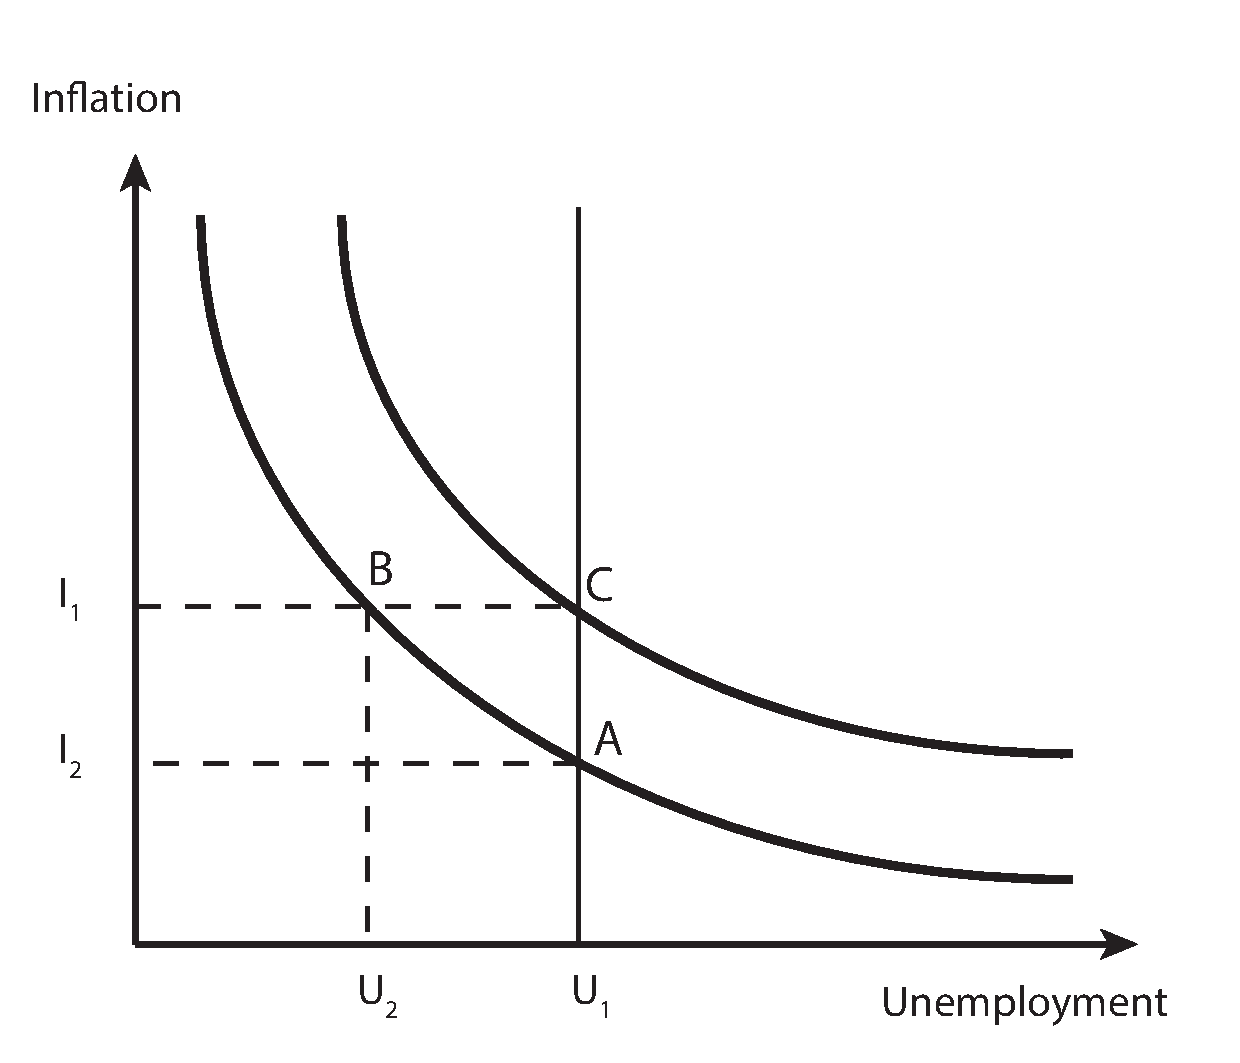
\includegraphics[width=0.75\linewidth]{Graphs/Phillips_curve_2}
	\caption{The Expectations-adjusted Phillips Curve}
	\label{fig:phillipscurve2}
\vspace{1.5cm}
\end{figure}


If a monetary policy decision temporarily inflates demand, firms react by producing more to accommodate the new interest in their products. In Figure~\ref{fig:phillipscurve2} this means a shift from point $A$ to point $B$ with unemployment being reduced from $U_1$ to $U_2$. Employers interpret this new demand as a cue to hire new workers, which in turn increases nominal wages. For workers this appears as an upward shift of their real wages in the industries that benefit first from the change in inflation rate.

As this process ripples through the economy the change in demand eventually pushes up wages to match the original change and the real wages return back to the original level. The shock has then died out as every agent has adjusted their expectations and unemployment returns back to the original as the Phillips curve shifts to incorporate the new level of inflation. In Figure~\ref{fig:phillipscurve2} this now means a shift from point $B$ to point $C$. Thus as the artificial and temporary demand shock has died out the unemployment returns to $U_1$ which is the Natural Rate.

The vertical solid line signifies the long-term relationship between the price level and unemployment. For any level of inflation there is a set of real factors such as technology, human capital, social institutions and such that determine the optimal potential level of production and a corresponding employment level. Monetary shocks on the other hand, only create modest ripples and temporarily tilt the curve.

In the 70's, the stagflation resulting from the oil crises gave credibility to the NRU story and ultimately the Nobel Price for Economics for Friedman. And when Ronald Reagan won the presidential elections in 1981, meant victory for the NRU and an economic policy doctrine of minimum interference.

In 1981, an avid supporter of the monetarist doctrine of minimal interference, Ronald Reagan won the presidential elections. This marked the beginning of the era of the NRU, as the dominant narrative defining economic policy.

The era of high inflation and low unemployment was over when the theory of NRU was put into practice. But a new problem was looming when the policy approach allowed higher levels of unemployment. In the textbook version of efficient clearing markets, the adjustment towards the natural rate happens automatically when the expectations and the production level are adjusted. But the social institutions governing the dynamics of employment are far more complex that this simple model suggests.

\vspace{2cm}

\subsection{The Hysteresis Hypothesis}

%\begin{displaycquote}{solow1990}
%	...I want to make the case that the labour market really is different. In particular I claim that it cannot be understood without taking acount of the fact that participants, on both sides, have well-developed notions of what is fair and what is not.
%\end{displaycquote}

The 1980s saw a rise of the laissez faire economics supported by the idea that active fiscal policy would only have temporary effects that would diminish as soon as the economy adjusted back to the natural level denoted by the NRU. Even though higher levels of unemployment were an obvious result of economic policy devoted to non-interference, the persistence was a surprise. \citep{nelson2007}

This was the concern of Olivier Blanchard and Lawrence Summers. They noticed, that unemployment showed path-dependant behaviour which would render the NRU-hypothesis and the non-interference policy approach non-applicable. Since it is not possible to achieve fully adjustable labour markets, downward rigidity of wages results in persistent unemployment as the market insiders (employed) and outsiders (unemployed) have different incentives. \citep{blanchard1986,blanchard1987} 

\cite{solow1990} proposed an alternative narrative to challenge the applicability of the theory of a naturally self adjusting equilibrium unemployment. He emphasized the relevance of the notion of fairness in a modern society, as a source of social conventions dictating labour market behaviour. Because of this fundamental intrinsic characteristic, labour markets may not function similarly to, for example goods markets as understood in the Walrasian general equilibrium framework. 

Employment and occupation are central to ones personal identity and the natural instinct for people to seek fair treatment makes selling and buying labour stand out from other markets. Solow suggests that labour market rigidities, which lead to difficulties in adjusting wages solely on the grounds of productivity are a product of the need to be treated fairly.

The desire to be treated fairly has two relevant consequences. First the reluctance to submit to lesser wage make it difficult for the firms in the economy adjust their production after negative shocks. Secondly the productivity of the employee is susceptible to effects of the workers perceived treatment. \citep{adams1962}

Trade unions and unemployment insurance systems may be responsible for a lot of the institutional obstacles to efficient wage adjusting labour markets. But it is plausible that the notion of fairness as an intrinsic property of a developed society is the fundamental cause. Solow \citeyearpar{solow1990} points out that merely acknowledging the existence of such force, makes it  necessary to address in the formulation of a complete theory on labour economics.

The more general theory on labour markets requires taking into account that such forces are at play that cannot be completely captured with the same tools as for markets for apples for instance. The idea that social institutions may play a role in labour market dynamics go beyond the need for justice. Other causal paths for the hysteresis hypothesis to be plausible are, for instance, the impairing effect of unemployment on workers skills \citep{pissarides1992} and the more general social exclusion that may result from an unemployment spell \citep{kieselbach2003}. Both of which lead into a situation where a portion of the labour force is rendered unproductive.

Long-term unemployment as a result of high levels of unemployment due to temporary negative demand shocks might also be solely enough as a source of hysteresis \cite{verho2014}. The duration structure and dynamics governing employment decisions conditional on the history of the applicant offer several interpretations that allow for strong persistence of unemployment on the aggregate especially in the absence of perfect information \citep{baker1992,krueger2014,eriksson2014}.

The mechanism behind unemployment is not as simple as the elementary equilibrium models suggest. The problems regarding asymmetric information, the social institution of fairness and duration dynamics provide us with several paths that lead to persistent unemployment. The NRU and hysteresis both provide narratives around which it is possible to build a coherent story to explain labour market behaviour and outcomes. It is however apparent that the conclusions are very different. That is why an empirical investigation is needed in order to uncover the relevance of persistence of unemployment.

\vspace{2cm}

\subsection{NAIRU as an empirical compromise}


It is not possible to fully review the whole story of NRU vs Hysteresis, without mentioning the Non-Accelerating Inflation Rate Unemployment(NAIRU). I will briefly introduce the concept as an empirical compromise and a possible theoretical synthesis between the contenders. 

Some scholars even argue that NAIRU is approximately a synonym to NRU \citep{ballmankiw2002}, but regardless of the exact definition, it is an important empirical tool. Even though the name NAIRU emerged later the concept was implied already by \cite{friedman1968}. 

As was discussed earlier the NRU is a level of unemployment that is realized if the economy is functioning at an optimal level of output considering current technology and institutional environment. Any downward deviation would result in an artificial acceleration of inflation according to the expectations adjustment process described in the previous two sections.

This general idea provides the possibility of approximating a level of unemployment that would be as close enough an approximation of NRU as possible. The standard starting point is to consider the formal definition of the NRU taken from \cite{friedman1968};

\begin{equation}\label{p-curve1}
\Pi = \Pi^e - \alpha(U-NRU) + v,
\end{equation}

where $\Pi$ is current inflation, $\Pi^e$ expected inflation and $(U-NRU)$ the output gap, $v$ a supply shock and $\alpha$ a positive scalar.

It has been shown that, in the short term, inflation tends to be a random walk process and thus a reasonable approximation for expected inflation is the present realized inflation ($\Pi^e = \Pi_{-1}$). Now the driving force of the shifts in the production gap is specifically unexpected inflation. \citep{ball2000, barsky1987}

Now it's possible to rearrange Equation \ref{p-curve1}
as

\begin{equation}\label{p-curve2}
\begin{split}
\Delta \Pi &= \alpha NRU - \alpha U + v  \Leftrightarrow \\
NRU + v/\alpha &= U + \Delta \Pi \alpha
\end{split}
\end{equation}

This arrangement provides sufficient means for estimating the $NRU$ term.  However there are still a number of identification issues to deal with, in addition to the interpretation difficulties resulting from previous assumptions.

First I assumed that current inflation is a reasonable approximation for expected future inflation. But the biggest problem to overcome when trying to estimate the $NRU$ is that $U$ and $v$ have to be uncorrelated. It is very difficult to imagine an external shock that does effect inflation but not unemployment or vice versa. The problem can be overcome to some extent by constructing instruments that separate the effects.

Fundamentally the identification problem that arises from the inseparability of inflation and current unemployment in the short term captures the essence of NAIRU as a half-way-point between NRU and Hysteresis narratives. The residual weight of $v$ could be hysteresis induced. The resulting estimate for NRU is found after assuming that hysteresis does not exist.

It is unlikely that the theoretical problems in estimating NAIRU will ever be solved. There are however numerous attempts at estimating it using technical compromises and additional covariates to reduce the contemporaneous correlation between $U$ and $v$. For example \cite{ballmankiw2002} use a straightforward method of applying a Hodrick-Prescott(HP) smoothing function to the right side of second line in Equation \ref{p-curve2}. They try to come with a time-varying NAIRU estimate for the US between 1960 and 2000 illustrated in graph \ref{ballmankiwNAIRU}. In their analysis it is assumed that $NRU$($U^*$ in the graph) varies over time but is relatively smooth. The size of the smoothing parameter of the HP filter $\lambda$ determines the magnitude of variation allowed for $NRU$.

In this chapter, I gave a review of the historical and theoretical background to the dichotomy of NRU vs Hysteresis. I also presented the NAIRU as a empirical and theoretical compromise between the two narratives. The NAIRU and the intrinsic problems in estimating it provided a great way to emphasise the complementary nature of the question around the NRU and Hysteresis. Next I will proceed to setting the groundwork to my own analysis by reviewing the relevant empirical literature.

\begin{figure}
\centering
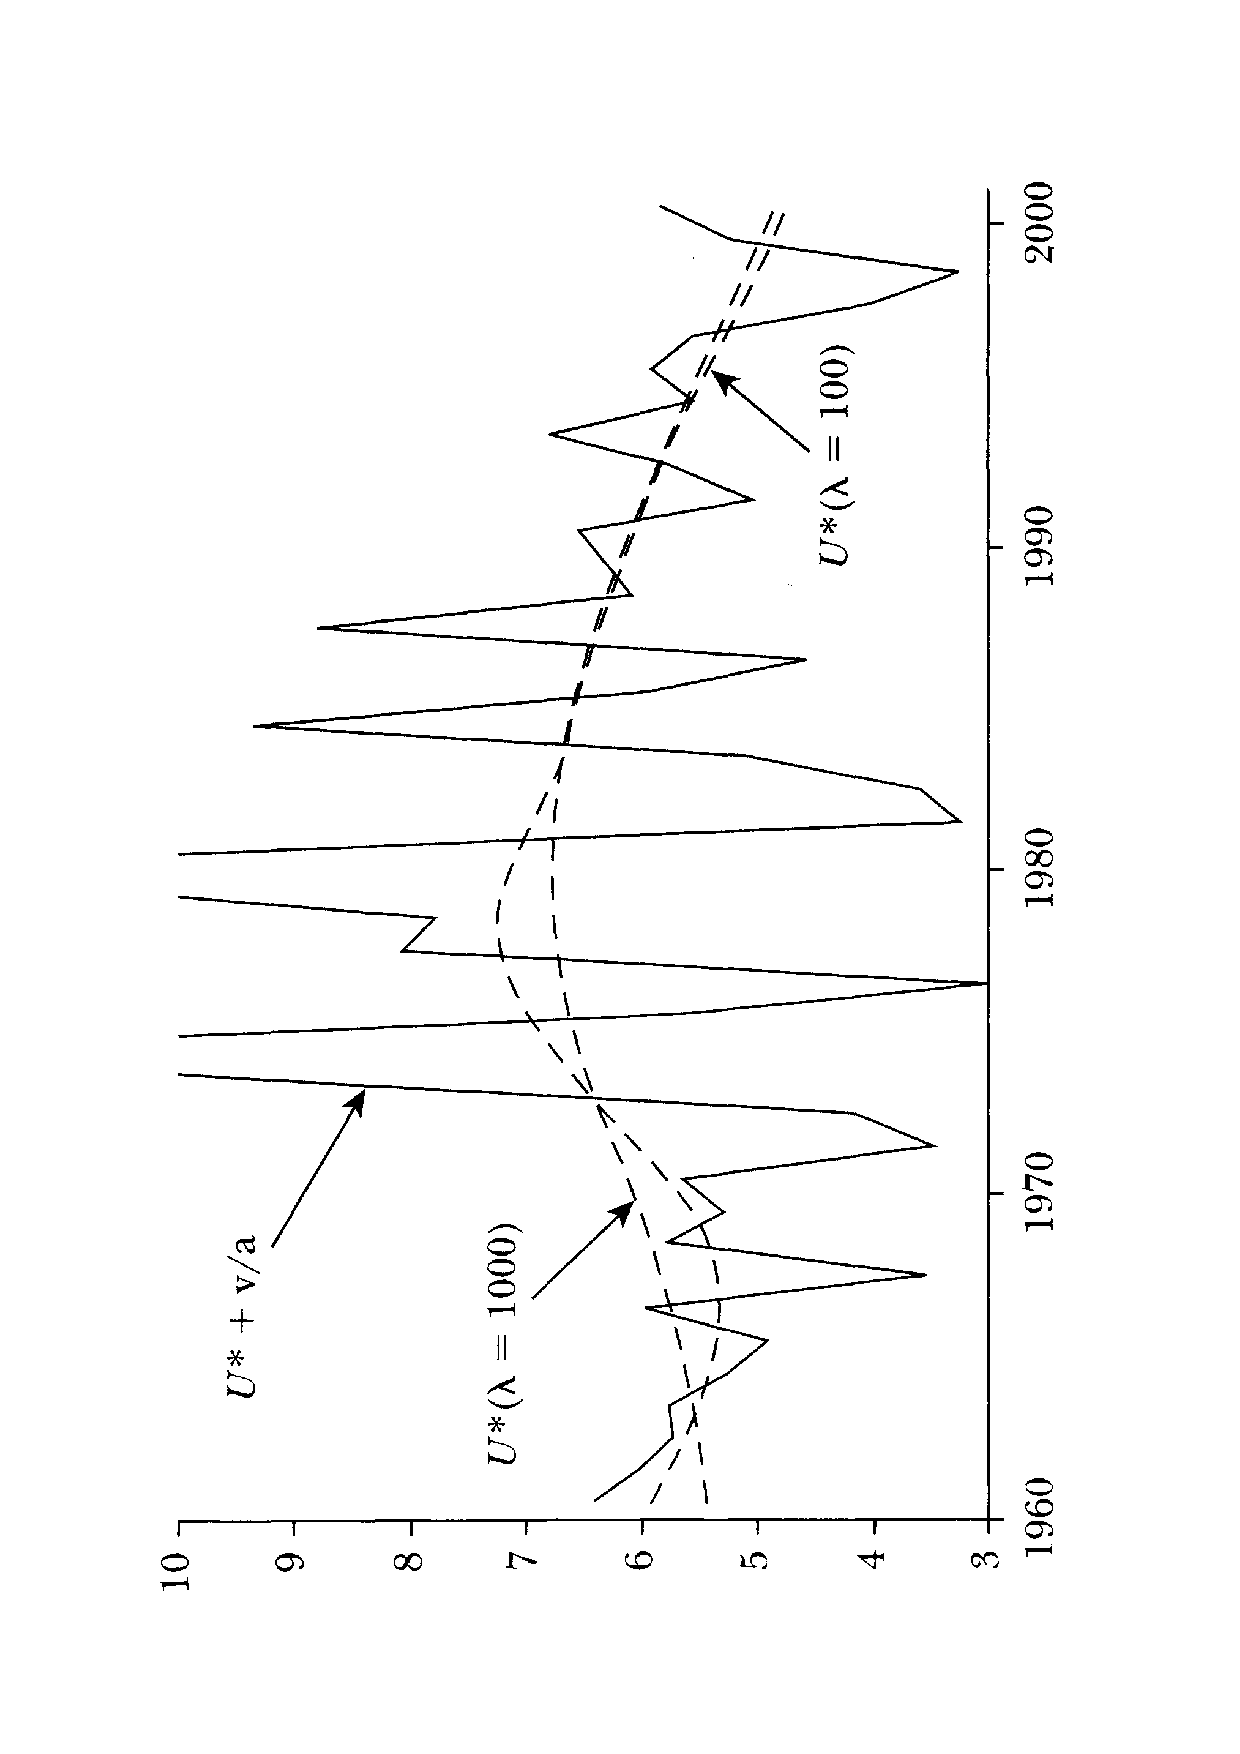
\includegraphics[width=0.8\linewidth,angle=-90]{Graphs/ballmankiwNAIRU}
\caption{Time Varying NAIRU 1960-2000 in the US. \citep{ballmankiw2002}}
\label{ballmankiwNAIRU}
\end{figure}
 

\clearpage
\section{Review of Empirical Literatrue}

In the previous chapter, I introduced the history of the theoretical approach to the question of hysteresis. Next I briefly review a selection of empirical research as well as elaborate on the specifics of my approach.

In addition to the overview of previous results I will motivate the gender decomposition approach by pointing out some differences in labour market behaviour between men and women that might affect the outcome of the test procedure.

Also, the magnitude of the results is discussed based on the shortcomings of the methodology as well as difficulties with isolating the phenomenon of interest. 

\vspace{2cm}

\subsection{Previous Empirical Studies}

There are several previous empirical studies that have tried to choose between the NRU and hysteresis stories. Typically, a null hypothesis of unit root is rejected for the United States but not for Europe. I have chosen to approach the question using established methodology in ADF and panel unit root tests. Running these tests separately for male and female unemployment series does provide insights on whether institutional differences between countries are more significant that behavioural differences between men and women. \citep{roed1996, leon2002}

Notably the methodology used by \cite{leon2002} is nearly identical to the one used in my analysis with the only major difference being the composition of the data and the time period. Although in addition to the IPS test, that \cite{leon2002} use, I also apply the MW test.

\cite{smyth2003} uses similar approach in testing for hysteresis in the Australian labour markets. The results are rather inconclusive with individual ADF tests for almost all territories failing to reject the null of hysteresis. Due to relatively similar institutional and cultural environment the results provide a good example of what to expect in my test setting.

The approach I have chosen seems gives more emphasis to the inter-temporal consistency of the data, than most previous studies. This translates to an assumption of less time needed for the NRU to shift due to structural causes.

Therefore the non-rejection of the null of unit root was expected across the countries and genders. Although a more qualitative interpretation of the test statistic values might provide a bit of new insight as well. Major relative differences in the statistic values between different studies and especially time-periods might suggest either major institutional shifts or provide insight to the power of the test procedures. 

\vspace{2cm}

\subsection{Motivation for the Gender Decomposition Approach}

I mainly chose to employ a panel approach to testing the persistence of European unemployment for reasons concerning the consistency of data over time. Monetary policy among other regimes and institutions, that determine the fundamental dynamics that affect labour market outcomes are susceptible to a variety of shocks and shifting currents. That is why it is necessary to determine a time span within which the institutional environment is comparable.

If it is not possible to accumulate information about the underlying process by extending the time frame the alternative is to take a closer look at the data. By expanding the data within the given interval by looking at the separate time series decomposed by gender, I have more information to feed into the tests. Labour market dynamics for men and women are somewhat different and it is necessary to consider the possibility that the underlying processes behind unemployment for different genders aren't perfectly comparable \citep{azmat2006}.

Furthermore, there is an abundance of research on the differences in unemployment dynamics between the genders. For instance women are more likely to exit the labour force when facing unemployment \citep{royalty1998, gonzalo2000}. Part of this difference can be explained by pregnancy. But as an overall tendency women tend to choose non-participation over unemployment more than men. That in turn lowers the overall unemployment rate.

The gender pay gap as well as unemployment gap are also explained by cultural and historical reasons forcing differences in education level attained and type of career pursued. It is very difficult to fully differentiate between gaps induced by job type, profession, education level or any other factor besides gender. \citep{azmat2006}

Women also tend to be employed by the public sector more than men mostly due to the fact that a lot of female dominated professions, such as healthcare professionals, teachers and occupations in the social services sector, are mostly employed by public entities. These industries may not be as susceptible to demand driven shocks as private sector jobs.

Another relevant difference is the higher likelihood for women to be employed part-time and the gender wage gap. It is a possible source of differences in unemployment dynamics that women are more flexible and willing to accept work at worse conditions. \citep{arulampalam2007}

Policy responses to realized gender gaps and other adverse differences in labour market outcomes for men and women are to be taken into account as well. The wage setting mechanism and institutional responses to providing women with equal opportunities differ a lot across the Eurozone countries. All these factors affect the magnitude and direction of the possible gender differences. \citep{blau2003}

To conclude, the decision to decompose the unemployment data by gender is a practical solution to a problem of technical nature. By finding significant differences in the dynamics of unemployment based on gender it is possible to provide some insight into the significance of these differences.

\vspace{2cm}

\subsection{Economic Policy Regimes and Time Frame of the Analysis}

Determining the time frame of European integration and structural shift towards the present system in terms of monetary and economic policy is surely open to debate. I will however do my best to provide as good a motivation for my choice as possible.

It is not possible to determine a strict starting point to a time frame within which I could confidently claim consistency from the perspective of my analysis. Thus I am forced to submit to good faith and take into account the possible bias brought by the shift in structural circumstances within the timespan of the analysis.

I have decided to use data starting from the year 1998 for two main reasons. First, it marks the beginning of the third stage of the EMU integration process that started in 1992 and can be identified as the beginning of the official unified monetary policy regime executed by the European Central Bank (ECB). Secondly it is the starting year of the official quarterly statistics within the LFS and thus ensures homogeneous methodology concerning data collection across the relevant countries as well as uniform availability.

The main components of policy circumstances relevant to the data generating process of unemployment are monetary policy, fiscal policy and labour market institutions. 

Monetary policy is the most straightforward of the three to examine. The ECB is responsible for executing monetary policy in the Eurozone. Although the effects of chosen policy might differ across the currency union it is clear that all countries inside it are under the same regime. 

The Maastricht Treaty is quite explicit in determining the main objective of the ECB:

\begin{displaycquote}{maastricht}
The primary objective of the ESCB shall be
to  maintain  price  stability.  Without  preju-
dice to the objective of price stability, the
ESCB  shall  support  the  general  economic
policies in the Community with a view to
the  achievement  of  the  objectives  of  the
Community as laid down in Article 2. The
ESCB  shall  act  in  accordance  with  the
principle of an open market economy with
free competition, favoring an efficient allo-
cation  of  resources,  and  in  compliance
with  the  principles  set  out  in  Article  3a.
\end{displaycquote}

Maintaining price stability and supporting stable economic performance of the Eurozone, should result in minimal business cycle variation. And in the absence of major shocks a stable unemployment levels near the NRU.

Whether the ECB has been successful or not I am inclined to assume that the policy decisions made within it's mandate has had a stabilizing effect on the Eurozone economy. Also the application of uniform monetary policy should result in convergence of institutional environment as has been observed \citep{agresti2001}. 

Fiscal policy and labour market institutions are under the control of national governments and their convergence is much harder to show.

In order to qualify for the single currency each member state has to commit to a set of rules aimed at creating a foundation for disciplined fiscal strategy. These rules were made permanent after the Euro came into existence with the signing of the Stability and Growth Pact (SGP) in 1997. The SGP rules provide only the broadest boundaries within which the Eurozone economies still have a wide set of motives and means to exercise their own chosen fiscal strategy. \citep{iversen2016}

These historical developments and treaties should give all the necessary catalysts for the Euro countries to choosing aligned paths in terms of economic policy and development of labour market institutions. That should allow for consistent analysis of the underlying dynamics of labour market mechanisms on the aggregate as I have done. Even though in absence of a controlled test setting, ultimately we can never be sure of the level of comparability between any two countries.


\vspace{2cm}

\subsection{Implications and Magnitude of Results}

As mentioned in the previous section the main concern of monetary policy during the time period covered by my analysis has been to maintain stable inflation rate below, but close to, 2\%. Although after the present crisis that has seen the new problem of persistent inflation rate well below the target rate. This has triggered some unconventional monetary policy decisions by the European Central Bank(ECB), such as extended  liquidity  provision (LTRO) and the Securities Market Program (SMP). Though their scale and estimated impact might have been smaller than the equivalent for the Federal Reserve and Bank of England. \citep{pattipeilohy2013, eser2016}

All the measures have been applied in order to reinvigorate the economy and steer it back toward the natural rate and act as artificial catalysts for the NRU mechanism. Thus the possible rejection of the hysteresis hypothesis has to be evaluated bearing this in mind.

The effect of fiscal policy applied during this time and especially in the recent years across the 11 countries are very difficult to measure. That is another reason why the implications of this analysis should be taken with a grain of salt. I do not intend to draw any far reaching conclusions on the precise mechanics at play but merely point out the existence of an issue to be addressed.

Also we have to take into consideration the possibility that the magnitude of the present crisis might have had such significant real effects to the economy that the Natural Rate has shifted as a result. This question brings us to the very core of the whole dichotomy of NRU versus hysteresis. The two explanations may be the polar opposites in a theoretical setting but practically indistinguishable in reality. Ultimately there is no way we can fully reject either one as a theoretical concept but rather evaluate their relative significance in a given structural and political setting.

The test setting used in this study is most likely rigged towards the non-rejection of the hysteresis hypothesis for two main reasons. First the time frame used because of the structural comparability means the power of the test is relatively low. And secondly because the possible rejection of the hypothesis can be interpreted as a success for the monetary policy applied by the ECB. This has to be taken into account when considering the implications of the results.

Despite it's shortcomings the unit root test employed in this study does give some relevant insight into the effectiveness of fiscal policy. If indeed the hysteresis narrative is deemed more suitable to describe developments of unemployment in the European economy then the doctrine of non-intervention cannot be justified by the mean reverting properties of unemployment. This in turn offers at least some credibility to demands of active and at times aggressive counter cyclical fiscal policy in order to maintain sufficient levels of aggregate demand. 

Regardless of the outcome of the tests what fundamentally matters is the magnitude of persistence. If unemployment is not characterized by an integrated time series model but exhibits impulse response half-lives measured in decades the policy implications are the same. That is why I urge the reader to take a holistic approach when reading into the implications of the result I present an allow the different sides of the story to complement each other.



\clearpage
\section{Data and descriptives}

The main data set I'm using, consists of quarterly unemployment levels decomposed by age groups and sex. The data are obtained from the Harmonized Unemployment Rate(HUR) dataset within the Short-Term Labour Statistics database published by \cite{oecdSTLABOUR}. The data have been collected by the National Statistics Institutes under the coordination of the European statistics agency Eurostat. Gathering the data has been carried out by surveys within the Labour Force Survey program (LFS).

All the data are acquired using the OECD Application Programming Interface(API) \citep{rOECD} for the R statistical program \citep{rBASE}. The decision to use the OECD as a middleman is based on the availability of the seasonally adjusted series in the same database, as well as the excellent overall usability of the OECD API.

The LFS is a European wide cross-sectional and longitudinal household sample survey gathered by the National Statistics Institutes. It consists on a vast database on labour force participation and a wide variety of background information on the survey participants. The survey is conducted with a questionnaire, collected by the national agencies under unified definitions in order to ensure consistency and comparability across participating countries and time. \citep{eurostat2009}

The quarterly unemployment rates used in this study are based on the following definition of unemployment: 

\begin{displaycquote}{tyovoimatutkimus2016}
	A person is unemployed if he/she is without work during the survey week, has actively sought employment in the past four weeks as an employee or self-employed and would be available for work within two weeks. A person who is without work and waiting for an agreed job to start within three months is also classified as unemployed, if he/she could start work within two weeks.
\end{displaycquote}

The HUR dataset consists of the base unemployment rate and the seasonally adjusted alternative that I have decided to use for the analysis. Due to high rates of seasonal variation a simple AR model would not have sufficed. Also the standard methods for adjusting for deterministic seasonal variation make the interpretation of the results more difficult.

\begin{figure}
\vspace{1.5cm}
\centering
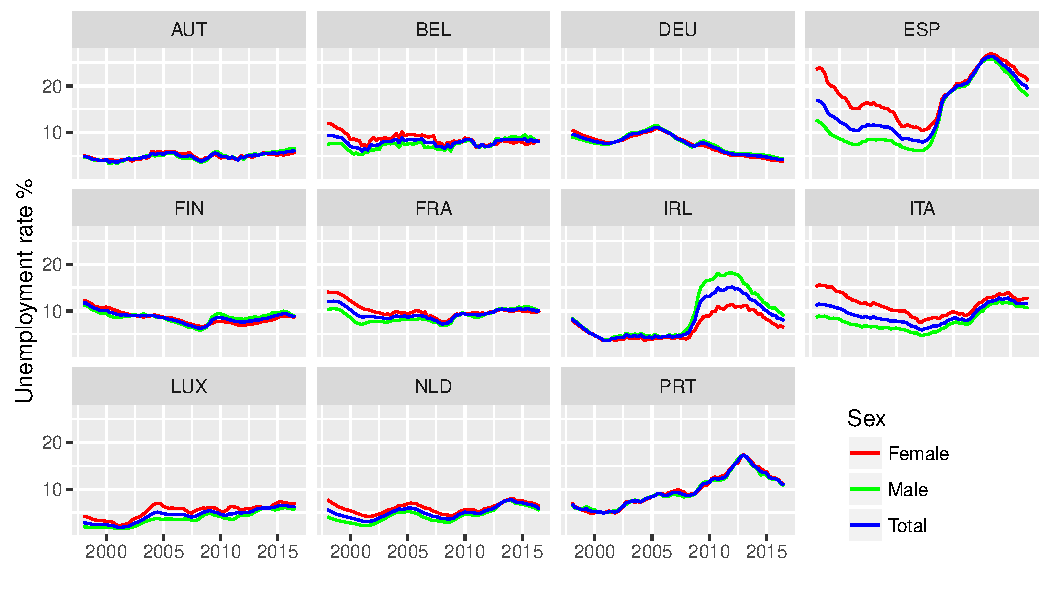
\includegraphics[width=0.9\linewidth]{Graphs/STSA_FE_MA_TT_facet}
\caption{Harmonized Unemployment Rates by Country and Gender.\cite{oecdSTLABOUR}}
\label{fig:stsafemattfacet}
\vspace{1.5cm}
\end{figure}


The seasonal adjustment method used by the OECD is a two stage process implemented with Demetra+ software. It is a combination of an ARIMA-based adjustment method by \cite{TRAMO} and a signal extraction procedure by \cite{SEATS}. As is clear from Figure \ref{ST_STSA_facet} for the most part the adjustment does not alter the series much except for Finland and Italy where consistent deterministic seasonal variation is present.

\begin{figure}
\vspace{1.5cm}
\centering
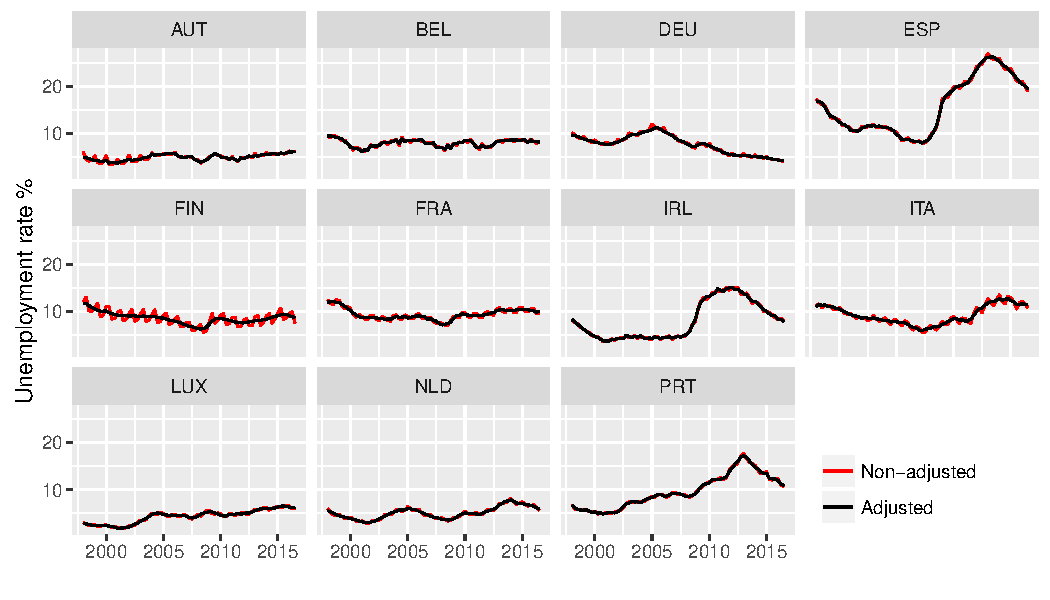
\includegraphics[width=0.9\linewidth]{Graphs/ST_STSA_TT_facet}
\caption{Original unemployment rates from the LFS and the seasonally adjusted.\cite{oecdSTLABOUR}}
\label{ST_STSA_facet}
\vspace{1.5cm}
\end{figure}



Empirical autocovariance plots depicted in Figure \ref{STSA_ACF_facet} revel strong correlation with high lag order with all the countries in the analysis. The graphs are all relatively smooth, which is why an AR process is likely to capture most of the relevant dynamics.

Spain, Portugal and Ireland especially exhibit obviously high levels of persistence but the case isn't as clear with the rest of the countries.

\begin{figure}
\vspace{1.5cm}
\centering
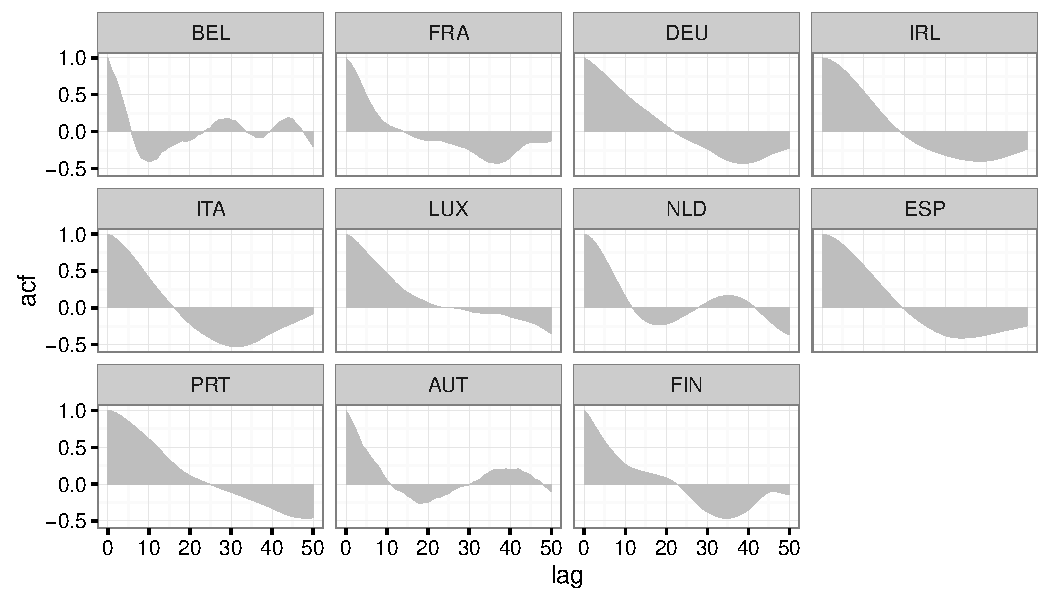
\includegraphics[width=0.9\linewidth]{Graphs/STSA_TT_ACF_facet}
\caption{Empirical autocovariance functions of seasonally adjusted aggregate unemployment rates.\cite{oecdSTLABOUR}}
\label{STSA_ACF_facet}
\vspace{1.5cm}
\end{figure}

If we look at the plots of first difference series in Figure \ref{STSA_diff_facet} it is quite obvious that for all countries included the time series are at least weakly stationary. Similar observations can be made about the time series decomposed across genders. See Appendix \ref{extradescriptives} for additional graphs.
     
The labour market participation rates plotted in Figure \ref{LFPR}, show obvious convergence between genders but also a distinct difference in levels. These data are also from the LFS published by \cite{oecdLFS}. Whereas the gender differences cannot be reduced to the participation rates, they illustrate the systematic pattern across all countries. 

\begin{figure}[H]
\vspace{1.5cm}
\centering
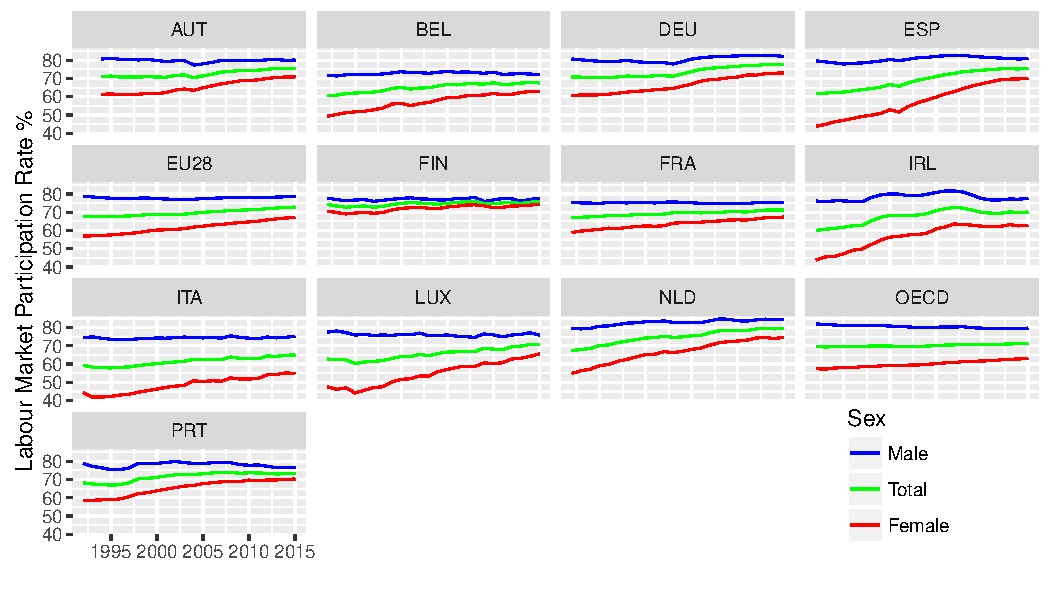
\includegraphics[width=0.9\linewidth]{Graphs/LFPR_FE_MA_TT_facet}
\caption{Labour Market Participation Rate. \cite{oecdLFS}}
\label{LFPR}
\end{figure}
                                     
\begin{figure}[H]
\centering
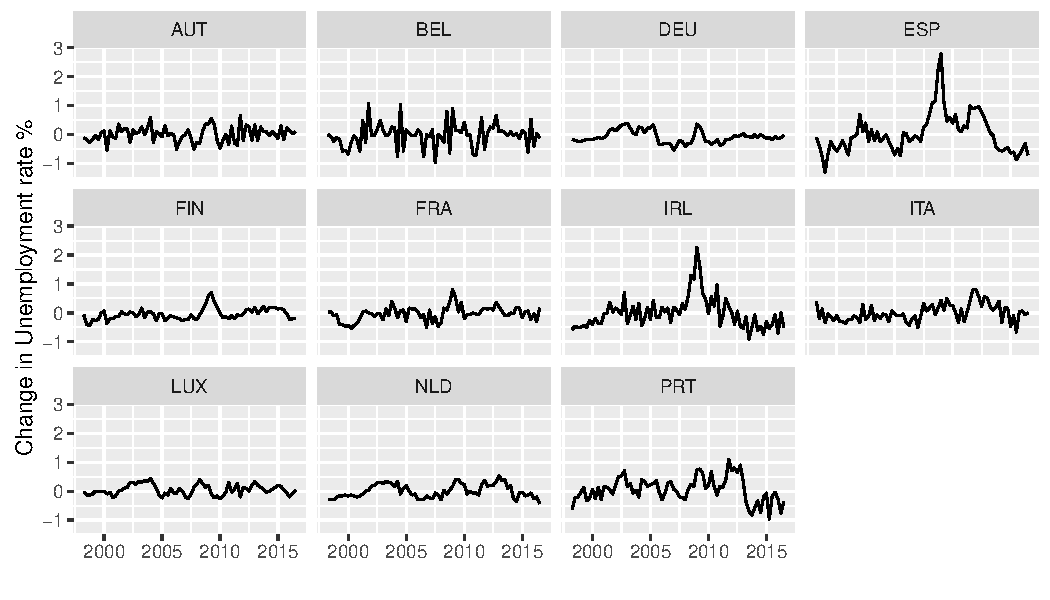
\includegraphics[width=0.9\linewidth]{Graphs/STSA_TT_diff_facet}
\caption{Rate of change in the quarterly seasonally adjusted unemployment rate. \cite{oecdLFS}}
\label{STSA_diff_facet}
\end{figure}

In this section I introduced the data used in the econometric analysis. Also, gender differences in labour market participation rate were briefly discussed. The next section introduces the econometric apparatuses employed in the mechanical part of this thesis.

\clearpage
\section{Statistical Model and Test Procedure}

In this chapter I will introduce the necessary methodological concepts applied in the study. Most of the methods are well established and are commonly accepted and might not require as thorough introduction as I have chosen to present. However, in order to maintain consistency I have decided to explicitly introduce every step of the way.

Consider an autoregressive model of order $p$, 

\begin{equation}
U_{t,i,g} = \delta_{i,g} + \theta_{1,i,g} U_{t-1,i,g} + \theta_{2,i,g} U_{t-2,i,g} + ... + \theta_{p,i,g}U_{t-p,i,g} + \epsilon_{t,i,g} ,
\end{equation}

where $U_{t,i,g}$ is the unemployment level for country $i$, gender $g \in {m,f,t}$ (for male, female and total) at time $t$, $\delta_i$ is the intercept term, and $\theta_{i,j}$ the coefficients corresponding to the country $i$ and lag $j$. Instead of unemployment levels, it is favourable to use unemployment rates in the analysis because considering possible dynamics in the labour force levels complicates the analysis and the clarity of results. In addition to this, the use of rate $\frac{U}{N}$, where $N$ is the size of the labour force, presents a problem for interpreting the results since the rate only deviates within the unit interval $[0,1]$. What is more, a bound process may not be truly considered a random walk even if a unit root is present. That is why a logit transformation

\begin{equation}
u_{t,i,g} = \log\bigg(\dfrac{U_{t,i,g}/N_{t,i,g}}{1-(U_{t,i,g}/N_{t,i,g})}\bigg)
\end{equation}

is applied before estimating the model. The transformed variable is denoted by lower case $u_{t,i} \in \mathbb{R}$ hereafter. Now the variable of interest is unbounded and the model is redefined as

\begin{equation}
 u_{t,i,g} = \alpha_i,g + \beta_{1,i,g}u_{t-1,i,g}+...+ \beta_{p,i,g}u_{t-p,i,g} + \epsilon_{t,i,g}
\end{equation}

%And the same process with the lag polynomial notation
%
%\begin{equation}
%\beta(L)u_{t,i,g} = \epsilon_{t,i,g}
%\end{equation}

The process $u_{t,i,g}$ is a unit root process if one of the roots of the lag polynomial is unity. That condition is satisfied if 

\begin{equation} \label{eq:1}
1-\beta_{1,i,g} - \beta_{2,i,g} - ... - \beta_{p,i,g} = 0  \text{ or if } \beta_{1,i,g} + ... + \beta_{p,i,g} -1 =0
\end{equation}

The expression in equation \ref{eq:1} can be rewritten as

\begin{equation}\label{ADFregression}
\Delta u_{t,i,g} = \alpha_{i,g} + \rho_{i,g} u_{t-1,i,g} + \sum_{j=1}^{p_{i,g}}\gamma_{j,i,g}\Delta u_{t-j,i,g} + \epsilon_{t,i,g} ,
\end{equation}

where $\rho_{i,g} = \beta_{1,i,g} + ... + \beta_{p,i,g} -1$. Now if I estimate this regressions the test on the significance of $\rho_{i,g}$ is a test for a unit root, usually referred to as the Augmented Dickey-Fuller test of order $p_{i,g}$ $(ADF(p_{i,g}))$. The order $p_{i,g}$ is selected using a standard information criterion procedure. First 8 different models are estimated using a standard OLS estimator with the first model including only 1 lag, the second two lags and so forth. Then the Akaike Information Criterion (AIC, equation \ref{AIC}) is calculated for each model and the one with the smallest value is selected.

\begin{equation} \label{AIC}
AIC = n \log\bigg(\dfrac{RSS}{n}\bigg) + 2 k , 
\end{equation}

where $RSS$ is the residual sum of squares and $k$ the number of lags.

After the selection algorithm is applied and the appropriate lag order is selected for all $i$ and $g$ the regression model in Equation \ref{ADFregression} is estimated. A hypothesis test on the coefficient $\rho$ is a standard t-statistic that has limiting distribution for finite samples that are non-standard as noted by \cite{dickey1981}. The critical values for the statistic are taken from the tables provided by \cite{dickey1981}.

The low power of the ADF-test is a well known issue especially when analysing time series' of limited length as we are forced to do \citep{harris1992, hoang2006}. In order to improve validity of unit root testing a number of panel tests have been devised to pool information from several time series with a comparable data generating process. In economic applications the most used ones are probably \cite{levin2002}(LL), \cite{im2003}(IPS) and \cite{maddala1999}(MW).

The LL test is ill-suited for macroeconomic analysis since it assumes that the alternate for the null hypothesis is such that all the series in the panel converge to the mean at the same rate. IPS and MW tests share the null hypothesis that all the series in the panel are unit root, against the alternative that at least some of the series are mean-reverting but not necessarily at the same rate. Formally for the panel tests which are calculated for each gender separately\footnote{Subscript $g$ omitted from hereon where possible, to improve readability}:

\begin{equation}
\begin{split}
&H_0: \rho_{i} = 0, \forall i,\\
&H_1: \rho_{i} < 0, i = 1,2,..N_1, \rho_{i} = 0, i = N_1,...,N
\end{split}
\end{equation}

Rejection of the null is thus proof that there is reason to assume that for at least some countries the unemployment series are characterized by a weakly stationary process. In other words the panel test is a way of reinforcing a rejection with the usual ADF test.

The statistic for the IPS test is defined by \cite{im2003}, as

\begin{equation}
\hat{t}_{IPS,g} = \dfrac{ \sqrt{N}(\bar{t}_{N,T}-N^{-1} \sum_{i=1}^{N} E[t_{i,T}(p_i)|\rho_i=0])  }{\sqrt{ N^{-1} \sum_{i=1}^{N}Var[t_{i,T}(p_i)|\rho_i=0]   }} \sim N(0,1) ,
\end{equation}

where $\bar{t}_{N,T}$ is the average of the $ADF(p_{i,g})$ test statistics over $N$ cross-sections (in this test setting executed in my thessis, $N=11, \forall g$). $E[t_{i,T}(p_i)|\rho_i=0]$ is the mean and $Var[t_{i,T}(p_i)|\rho_i=0]$ the variance of $\bar{t}_{N,T}$, all tabulated by \cite{im2003} for different lag lengths and orders.

Properties of the IPS test has been investigated by several authors and especially the susceptibility of the size and power of the test to problems arising from cross-sectional correlation is a well known issue \citep{karlsson2000, hoang2006}. Monte Carlo analysis performed by \cite{hoang2006} provides tabulated values for the power and size for different $T$ and $N$. For $T=50$ and cross-sectional correlation of 0.25 the power of the test would be .972 for $N=100$, and .601 for $N=50$. The corresponding sizes are .004 and .002.\footnote{The cross-sectional residual correlations of the estimated $ADF(p_{i,g})$ regressions are tabulated in the Appendix \ref{CORRtables}}

The MW test takes a slightly different approach to aggregating the statistics. It accumulates the information gathered in the p-values of the $ADF(p_{i,g})$ test statistics.\footnote{Any other univariate unit root test could be used as well without any loss in generality.} The MW statistic is formally defined as:

\begin{equation}
p_{\lambda,g} = -2\sum_{i=1}^{N} \log \pi_{i,g} \sim \chi^2_{2N} , 
\end{equation}

where $\pi_{i,g}$ is the p-value of the $ADF(p_{i,g})$ test for country $i$ and gender group $g$. 

In conclusion the power of the test might be reduced by the apparent dependency of residuals across countries which has to be taken into account when interpreting the results. In addition to providing the test statistic values I will also look at the Impulse Response Functions(IRF) of the estimated univariate models of order $p_{i,g}$ of all combinations of countries and genders that reject the null at any usual confidence level. This provides some insight about the speed at which the model tends to return back to it's natural level in the absence of new shocks.


\clearpage
\section{Estimation results}

In this section I present the estimation results calculated using the procedure detailed in the previous chapter. First, I discuss the ADF statistic table and point out the main observations. Then I introduce the panel statistic values and move on to interpret the IRF graphs for the countries that reject the null of unit root hysteresis.

\begin{table}[H]\label{combinedADF}
\vspace{1.5cm}
\centering
\input{Tables/combined_ADFtable.txt}
\caption{Tabulated ADF statistic values and model orders}
\vspace{1.5cm}
\end{table}



%\begin{table}\label{maleADF}
%\centering
%\input{Tables/STSA_MA_ADFtable.txt}
%\caption{Tabulated ADF statistic values for male u nemployment}
%\end{table}

Based on previous empirical research reviewed in the first chapter, I did expect to see at most a few rejections of the null of hysteresis. But what is striking is the obvious difference between the genders. In Table \ref{combinedADF}, listing the ADF statistics for total, male and female unemployment, we can see that the only rejection of the null, in the male column, is at the 10\% confidence level for Netherlands. Considering the panel size of 11 in is quite possible that interpreting the result as significant would constitute an incorrect rejection of the null.

%\begin{table}\label{femaleADF}
%\centering
%\input{Tables/STSA_FE_ADFtable.txt}
%\caption{Tabulated ADF statistic values for female unemployment}
%\end{table}

However the corresponding column for female unemployment looks very different with four rejections at the 5\% significance level (Belgium,France, Netherlands, Finland). The difference between the two genders cannot be explained by a Type I error considering the sufficient size of the test discussed in the previous chapter. The likelier explanation is the differences in unemployment dynamics captured in this test.

%\begin{table} \label{totalADF}
%\centering
%\input{Tables/STSA_TT_ADFtable.txt}
%\caption{Tabulated ADF statistic values for total unemployment}
%\end{table}

Looking at the column with the same statistics calculated for unemployment aggregated across genders the picture is muddied again with only one clearly significant rejection(Belgium). Looking at all the three columns side by side it is easy to conclude that it is very likely that the mean reverting tendency of total unemployment is explained by the section of unemployed composed of female subjects. As I pointed out in the first chapter it is well documented that different genders have different responses to adverse economic conditions. And differences between countries in this respect is at least partly due to different social conventions as well as different rates of labour market participation for females.

\begin{table}\label{paneltable}
\vspace{1.5cm}
\centering
\input{Tables/panel_table.txt}
\caption{Panel test statistics}
\vspace{1.5cm}
\end{table}

The IRF graphs of the models that reject the null (male: Netherlands ; female: Belgium, France, Netherlands, Finland ; total: Belgium, France, Netherlands) are plotted in Figure \ref{IRFfacet}. While all the models show some persistence, half-life of the simple point estimate impulse response seems to be under 25 lags for all the models. That does suggest fast enough convergence to be considered truly mean reverting within a time frame that can be considered comparable. It is however a remarkably long time when put into context.

\begin{figure} \label{IRFfacet}
\centering
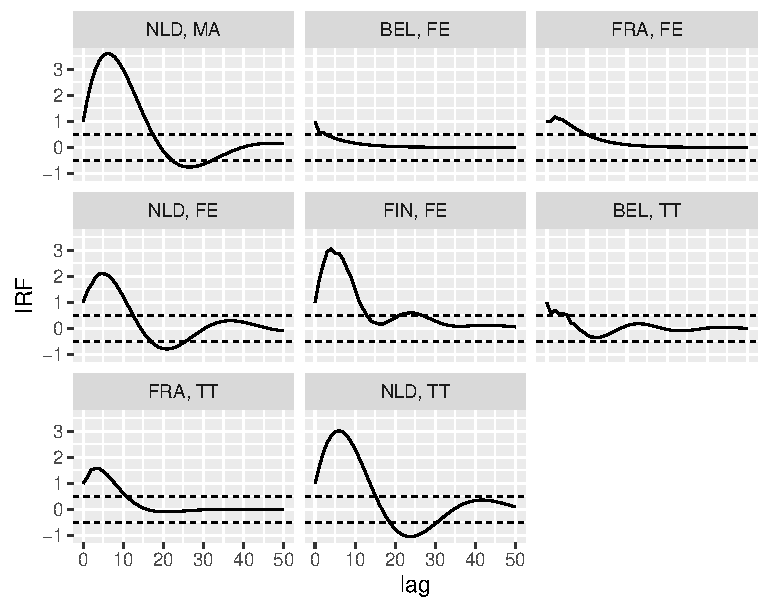
\includegraphics[width=0.9\linewidth]{Graphs/STSA_IRF_facet}
\caption{Impulse Response Functions for the countries and genders rejecting the null of unit root. Horizontal dashed lines at 0.5 and -0.5}
\label{fig:stsairffacet}
\end{figure}
%\begin{table} \label{IPStable}
%\centering
%\input{Tables/IPS_table.txt}
%\caption{IPS-statistics}
%\end{table}

In Table \ref{paneltable} I have listed the IPS and MW statistic values for male, female and total unemployment. If we first look at the IPS statistics, the results correspond with the deductions made with the individual ADF tests. The IPS statistics seem to confirm the explanatory power of the gender decomposition. It is even clearer that, looking at male unemployment alone it is not possible to reject the possibility of unit root persistence.

%\begin{table} \label{MWtable}
%\centering
%\input{Tables/MW_table.txt}
%\caption{MW-statistics}
%\end{table}

However the MW statistic (see Table \ref{paneltable}) does reject the null with very high significance for all gender groups. The statistic value is remarkably lower for male than female, even though the rejections is the only reasonable conclusion for both as well as the total unemployment. The strikingly different results between the two panel tests presents a inconvenient problem for my conclusions. The MW statistic value for all three groups is high enough to not leave any room for doubt; for some countries rejection of the null of unit root is highly likely. Whereas the IPS statistic would allow me to draw a very clear, but different, conclusion about the relevance of gender differences.

After calculating the statistics and realizing their implications, I felt that for consistency and transparency, I have no choice but to present them both. Instead of it being an inconvenience though I would like to see this superficial inconsistency as being an illustration of the complementary nature of the whole question of labour market behaviour and its study.

In this section of my thesis I presented the results of the econometric tests introduced previously. Most notably there seems to be a clear difference between male and female unemployment dynamics. Although based on the panel tests it seems plausible that at least some of the countries do follow a mean reverting unemployment path in the aggregate as well. The implications of these observations are discussed in the final section. I will also present the policy implications of the results in the context of the wider theoretical debate.

\clearpage
\section{Conclusions}

The results of the econometric tests introduced in this thesis revealed a sharp difference between genders. It seems that for several countries, the mean-reverting tendency of unemployment is driven by the behaviour of female participants alone. Overall it seems that the persistence of unemployment is very high in the Eurozone. Although the MW panel test rejects the possibility that all the countries exhibit unit root persistence in unemployment, it is fair to say that the mean-reverting tendency is definitely not dominant.

The existence of difference between genders is not surprising considering the differences in labour market behaviour for men and women, such as concentration to different industries and professions. All the countries rejecting the null of hysteresis have a relatively high levels of female labour market participation. Furthermore, the possibility that the null rejecting statistics are solely a result of female unemployed exiting the labour force cannot be ignored. Further research is therefore needed in order to gain additional insight to the story behind this finding.

It is possible that the institutional circumstances act as a catalyst that amplifies the behavioural differences. For instance, if we can show that the null-rejecting countries (Belgium, France, Netherlands and Finland) have also strong maternal support regimes that allow for easier family planning at the expense of long continuous careers the mean-reverting effect could be produced by women unemployed choosing motherhood instead of unemployment. 

Regardless of the exact dynamics that have generated these data, the most relevant interpretation to this finding is that differences between genders are more pronounced than differences between countries. All the contenders for relevant covariates require further investigation, and the main lesson to be learnt from the results of my analysis is that gender differences matter in the aggregate labour market outcomes.

Overall, despite the best efforts by the European Central Bank and national governments, unemployment is still elevated from the initial shock of the Great Recession. Apart from Belgium and France the null of unit root hysteresis cannot be rejected at the .05 significance level for total unemployment. These rejections are apparently all driven by the behaviour of the female half of the aggregate. Although the MW statistics do suggest that for at least one country a mean reverting model would be more accurate.

The policy implications of my results are two fold. First it is necessary for me to highlight the fact that external shocks producing elevated unemployment levels seem to be very persistent in the Eurozone. Long lasting effects of shocks in labour demand, in turn are either the result of ineffective policy response from the national governments and the Europen Central Bank or the nature of the shock itself. Whoever is the main culprit, the conclusion remains such that the current regime of institutions and policy mechanisms is not effective enough to deal with shocks of the magnitude we saw in the aftermath of the current financial crisis.

The second takeaway for policy makers is the observation that gender does matter in determining the labour market outcomes of Eurozone citizens. Even though the participation rates are on a convergent path, the issue of equality is not solved. 

Based on the analysis presented here, the NRU model does not seem to fit the Eurozone labour dynamics. Frictions and complexities, as elaborated in chapter 2, do seem to matter in such a magnitude that unemployment persists. This result is by no means conclusive, but does reinforce previous conclusions made on the topic. The analysis based on this paper should be complemented by a closer inquiry into the gender differences in labour market behaviour to reveal further insights on the topic.






\clearpage

\bibliographystyle{agsm}
	
\bibliography{gradu}


\clearpage


\begin{appendices}


\section{List of the countries in the analysis and their abbreviations }\label{countries}

The countries included in the analysis are the 11 original Eurozone countries. In order to make the graphs more readable I have used the official abbreviations for the country names.

\begin{tabular}{l r}
Austria & AUT \\
Belgium & BEL \\
Finland & FIN \\
France & FRA \\
Germany & DEU \\
Ireland & IRL \\
Italy & ITA \\
Luxemburg & LUX \\
Netherlands & NLD \\
Portugal & PRT \\
Spain & ESP \\
\end{tabular}

\section{Plots of decomposed time series}\label{extradescriptives}

In addition to the descriptives presented in chapter 4, here are some additional graphs. First the unadjusted unemployment time series with superimposed seasonally adjusted ones decomposed by gender, from the Harmonized Unemployment Rate (HUR) series from the Short Term Labour Market Statistics database, collected by Eurostat for the LFS.

Also the plotted autocovariance functions of the seasonally adjusted time series are presented here separately for female and male subjects.

And in order to rule out higher order unit root behaviour the first difference series is also added with separate plots for male and female subjects separately. Also calculated from the seasonally adjusted levels. 


\begin{figure}[H]

\centering
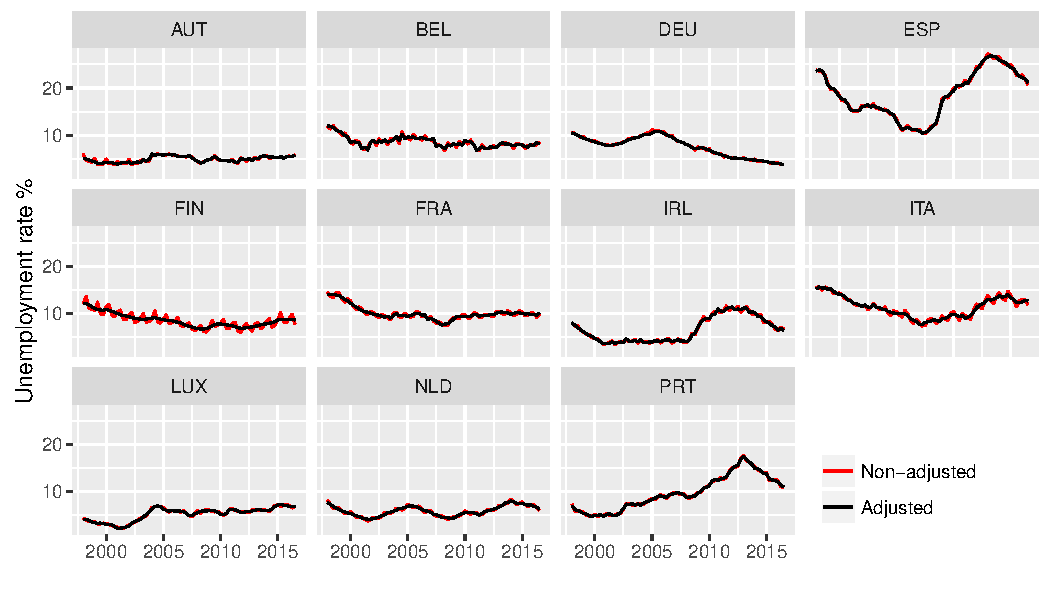
\includegraphics[width=0.8\linewidth]{Graphs/ST_STSA_FE_facet}
\caption{Original unemployment rates from the LFS and the seasonally adjusted for female subjects.\cite{oecdLFS}}
\label{ST_STSA_FE_facet}
\end{figure}

\begin{figure}[H]
\centering
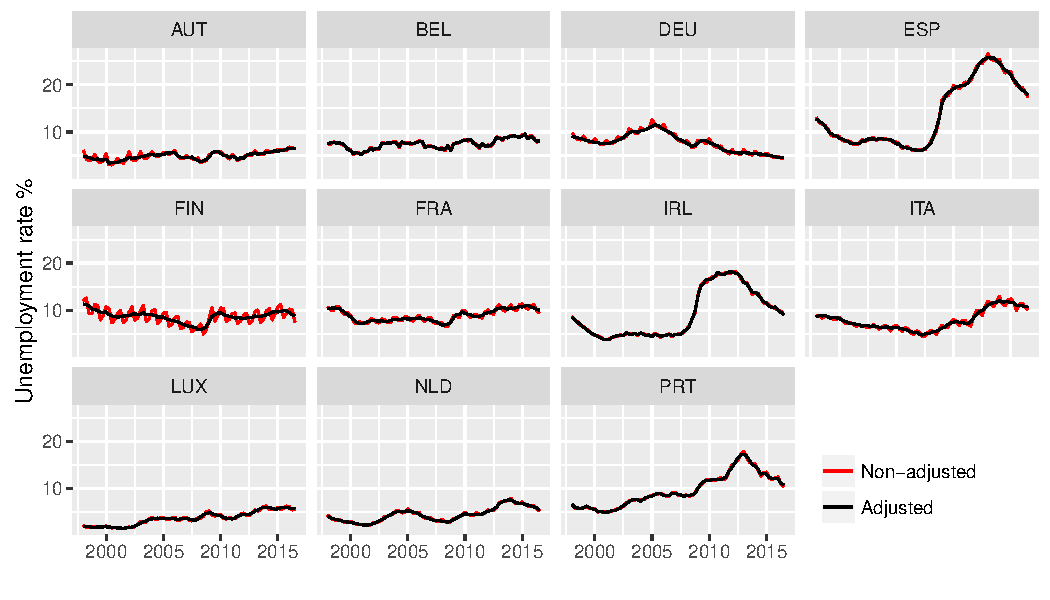
\includegraphics[width=0.8\linewidth]{Graphs/ST_STSA_MA_facet}
\caption{Original unemployment rates from the LFS and the seasonally adjusted for female subjects.\cite{oecdLFS}}
\label{ST_STSA_MA_facet}
\end{figure}

\begin{figure}[H]
\centering
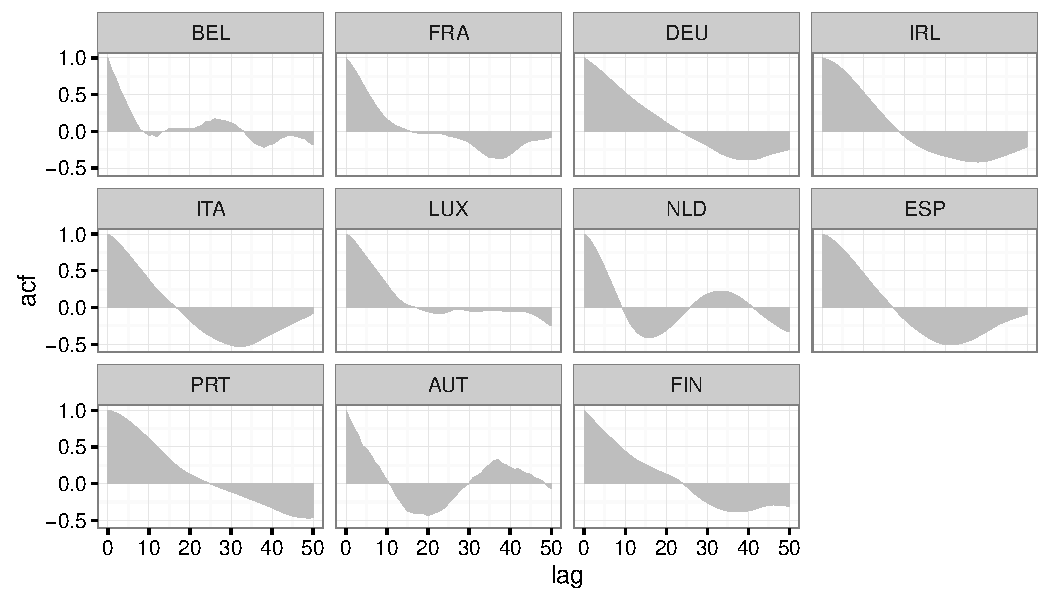
\includegraphics[width=0.8\linewidth]{Graphs/STSA_FE_ACF_facet}
\caption{Autocovariance functions of seasonally adjusted unemployment rates for female subjects.\cite{oecdLFS}}
\label{STSA_FE_ACF_facet}
\end{figure}

\begin{figure}[H]
\centering
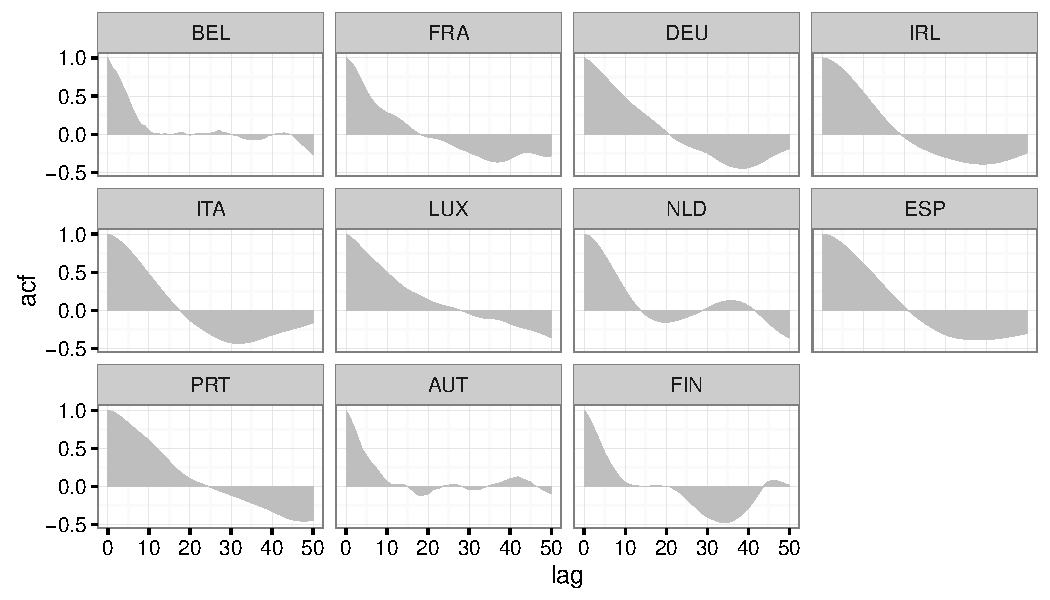
\includegraphics[width=0.8\linewidth]{Graphs/STSA_MA_ACF_facet}
\caption{Autocovariance functions of seasonally adjusted unemployment rates for male subjects.\cite{oecdLFS}}
\label{STSA_MA_ACF_facet}
\end{figure}

\begin{figure}[H]
\centering
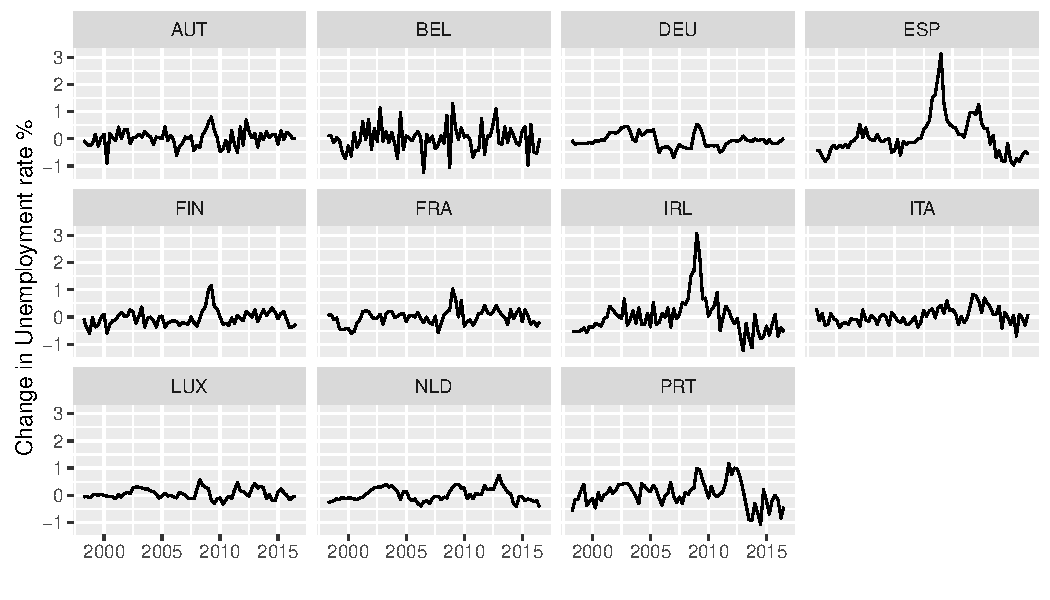
\includegraphics[width=0.8\linewidth]{Graphs/STSA_MA_diff_facet}
\caption{Rate of change in the quarterly seasonally adjusted unemployment rate for male subjects.\cite{oecdLFS}}
\label{STSA_MA_diff_facet}
\end{figure}

\begin{figure}[H]
\centering
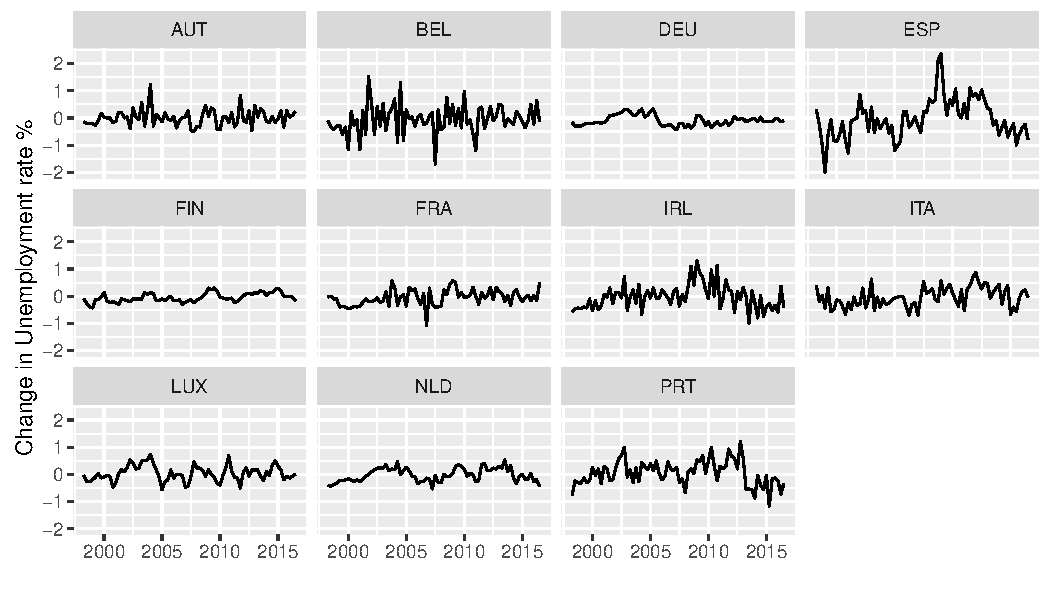
\includegraphics[width=0.8\linewidth]{Graphs/STSA_FE_diff_facet}
\caption{Rate of change in the quarterly seasonally adjusted unemployment rate for female subjects.\cite{oecdLFS}}
\label{STSA_FE_diff_facet}
\end{figure}

\clearpage

\section{Cross-sectional correlation coefficient tables of ADF residuals}\label{CORRtables}

This appendix contains tabulated correlation coefficients of the residuals of estimated models used in the analysis. These tables are provided for the reader to estimate the validity of the research strategy as strong cross-sectional correlation renders the power of the panel tests ineffective.




\begin{table}[H]
\centering
\input{Tables/STSA_MA_CORRtable.txt}
\caption{Cross-sectional correlation coefficients of ADF regression residuals for male unemployed}
\end{table}

\begin{table}[H]
\centering
\input{Tables/STSA_FE_CORRtable.txt}
\caption{Cross-sectional correlation coefficients of ADF regression residuals for female unemployed}
\end{table}

\begin{table}[H]
\centering
\input{Tables/STSA_TT_CORRtable.txt}
\caption{Cross-sectional correlation coefficients of ADF regression residuals for total unemployed}
\end{table}
\end{appendices}
\end{document}